\documentclass[../proyecto.tex]{subfiles}

\begin{document}
\chapter{Implementación}\label{chap:implementacion}

En este capítulo se describirá en profundidad como se ha realizado la implantación de la soluciones propuestas en el \autoref{chap:analisis_del_problema} tanto para el desarrollo del sensor como del servidor central. Divido en dos secciones principales, en la  \autoref{sect:impementacion_sensor} se describirá la implementación del sensor y en la \autoref{sect:impementacion_servidor_central} la del servidor central.\\

 \section{Sensor}\label{sect:impementacion_sensor}

Como se ha comentado en el análisis de tecnologías para la realización de este sensor se ha seleccionado el SoC ESP32, utilizando una placa de desarrollo ESP32 DevKitC de Espressif y para el desarrollo del código se ha elegido el \textit{framework} Arduino aunque para algunas funcionalidades de más bajo nivel se utilizarán librerías del \textit{framework} ESP-IDF.\\

Para la estructuración del código principal se ha utilizado la estructura básica de \textit{Sketch} de Arduino consistente en dos fases: \textit{Setup} y \textit{Loop}. La fase de \textit{Setup} solo se ejecutará una vez en cada encendido o reinicio del dispositivo y en ella se realizan las tareas de incialización del dispositivo. Una vez realizada la inicialización se ejecutará la fase \textit{Loop}, se trata de un bucle infinito en el que se definirá la lógica del sensor.\\

Durante la fase de inicialización el módulo ejecutará secuencialmente las siguientes tareas:
\begin{itemize}
  \item Generar identificador único utilizado para enviar las detecciones al servidor central.
  \item Conéctar a una red WiFi para sincronizar la hora mediante el prótocolo SNTP.
  \item Inicializar el escaneo Bluetooth.
  \item Inicializar el escaneo WiFi.
\end{itemize}

A continuación se realizará una breve descripción del código relacionado con la detección de las tramas Bluetooth y WiFi, y del procedimiento para su envío al servidor central.\\

Para realizar la detección de dispositivos Bluetooth se ha utilizado la librería \textit{BLEScan} incluida en las librerías de Arduino para el ESP32, esta librería crea una capa de abstracción sobre las librerías de BLE de ESP-IDF facilitándonos una API que se adapta a la mayoría de casos de uso al mismo tiempo que provee de métodos para ajustar y adaptar a más bajo nivel para casos más complejos.\\

Esta librería reduce enormemente la complejidad del código ya que además de simplificar la interacción con las librerías de \textit{ESP-IDF} nos proporciona otras ventajas como la posibilidad de registrar una función \textit{callback} asíncrona que será invocada cada vez que un dispositivo sea detectado.\\

En la función \textit{callback} se extraerá la dirección Bluetooth del anunciante y se guardará la fecha y hora de la detección en formato de fecha Epoch.\\

\begin{minipage}{\linewidth}
\begin{lstlisting}[language=C++, caption=Función \textit{callback} para el escaneo BLE, captionpos=b, frame=single]
class ble_advertised_device_cb: public BLEAdvertisedDeviceCallbacks {
    void onResult(BLEAdvertisedDevice advertisedDevice) {
        time_t now;
        time(&now);
        String bd_addr = advertisedDevice.getAddress().toString().c_str();
        ble_detected[bd_addr] = now;

        #if DEBUG == 1
        Serial.println();
        struct tm timeinfo;
        localtime_r(&now, &timeinfo);
        Serial.printf("Bluetooth detection: | MAC: %s ", advertisedDevice.getAddress().toString().c_str());
        Serial.print(" - Time: ");
        Serial.print(&timeinfo);
        Serial.println();
        #endif
    }
};Z
\end{lstlisting}
\end{minipage}

Para monitorizar el tráfico WiFi ha sido necesario utilizar funciones de la API de ESP-IDF ya que las librerías de Arduino no proveen la posibilidad de activar el modo promiscuo necesario para poder analizar todo el tráfico WiFi y no solo el dirigido a nuestro dispositivo.\\

La API de \textit{Networking} del ESP-IDF nos permite activar el modo promiscuo en la interfaz WiFi y además permite registrar una función \textit{callback} asíncrona que será invocada cada vez que un paquete es recibido, pero como se observó en el análisis del estándar WiFi para la detección de dispositivos solo necesitamos los paquetes de tipo \textit{management} y por tanto ejecutar el análisis del paquete con cada evento supondría una gran penalización en rendimiento, pero gracias a la función \textit{esp\_wifi\_set\_promiscuous\_filter} podemos establecer un filtro para determinar que tipo de paquetes dispararan la llamada a la función \textit{callback}, en concreto podemos utilizar el filtro \textit{WIFI\_PROMIS\_FILTER\_MASK\_MGMT}.\\

\begin{minipage}{\linewidth}
\begin{lstlisting}[language=C++, caption=Activación del modo promiscuo con filtrado, captionpos=b, frame=single]
const wifi_promiscuous_filter_t filter={.filter_mask=WIFI_PROMIS_FILTER_MASK_MGMT};
esp_wifi_set_promiscuous_filter(&filter);
esp_wifi_set_promiscuous_rx_cb(&Sniffer::sniffer_callback);
esp_wifi_set_promiscuous(true);
\end{lstlisting}
\end{minipage}

Las librerías de ESP-IDF nos proporcionan una estructura de datos para el almacenamiento del paquete recibido por la función \textit{callback} pero en esta estructura solo se define miembros para los metadatos de la capa de radio como el canal dónde se ha recibido el paquete o la fuerza de la señal, sin embargo el propio \textit{frame} se presenta como un simple puntero a los datos en bruto, esta estructura por tanto resulta ineficiente para la manipulación de los campos que necesitamos y es necesario definir nuestras propias estructuras de datos para almacenar la trama IEEE802.11 de tipo \textit{management}.\\

\begin{minipage}{\linewidth}
\begin{lstlisting}[language=C++, caption=Estructuras de datos para almacenamiento de las cabeceras IEEE802.11 , captionpos=b, frame=single]
struct frame_control {
    unsigned protocol_version:2;
    unsigned type:2;
    unsigned subtype:4;
    uint8_t stuff;
} __attribute__((packed));

struct iee80211_header {
    struct frame_control frame_control;
    uint16_t duration_id;
    uint8_t address_1[6];
    uint8_t address_2[6];
    uint8_t address_3[6];
    uint16_t seq_ctrl;
};
\end{lstlisting}
\end{minipage}

Una vez definidas las estructuras de datos necesarias podemos realizar el análisis de la trama en busca de la dirección de la estación emisora, esta lógica se define dentro de la función \textit{callback} descrita anteriormente. En esta función se realizará la extracción de la dirección MAC y se almacenará junto a la fecha y hora de detección en formato de tiempo Epoch.\\

\begin{minipage}{\linewidth}
\begin{lstlisting}[language=C++, caption=Función \textit{callback} para el modo promiscuo , captionpos=b, frame=single]
void ICACHE_FLASH_ATTR Sniffer::sniffer_callback(void *buff, wifi_promiscuous_pkt_type_t type)
{
    if (type == WIFI_PKT_MGMT) { //Maybe unnecessary after filter
        // Obtenemos el
        const wifi_promiscuous_pkt_t *packet = (wifi_promiscuous_pkt_t *)buff;

        struct Sniffer::iee80211_header *header = (struct iee80211_header*) packet->payload;
        if (header->frame_control.type == TYPE_MANAGEMENT
            && header->frame_control.subtype == SUBTYPE_PROBE_REQUEST) {
              time_t now;
              time(&now);
              // The second address in MAC header is the transmitting station.
              uint8_t *addr = header->address_2;
              char mac_addr[18];
              sprintf(mac_addr, "%02x:%02x:%02x:%02x:%02x:%02x", addr[0], addr[1], addr[2], addr[3], addr[4], addr[5]);
              sta_detected[String(mac_addr)] = now;
              #if DEBUG == 1
                Serial.println();
                struct tm timeinfo;
                localtime_r(&now, &timeinfo);
                Serial.print( "WiFi detection | MAC: " + String(mac_addr) );
                Serial.print(" - Time: ");
                Serial.print(&timeinfo);
                Serial.println();
              #endif
        }
    }
}
\end{lstlisting}
\end{minipage}

Una vez lanzados los procesos asíncronos de detección en el bucle principal se comprobará si el número de detecciones realizadas supera el umbral establecido, esta comprobación se realiza en intervalos de 200 ms y una vez alcanzado el umbral la detección se detendrá temporalmente para dar paso al envío de las detecciones al servidor central, la detención del escaneo es necesaria ya que el módulo no puede estar en modo promiscuo y en modo estación simultáneamente. El umbral establecido es de 100 detecciones, este umbral ha sido calculado en base a las limitaciones de memoria del módulo y a minimizar el tiempo de parada que será necesario para el envío de las detecciones.\\

\begin{minipage}{\linewidth}
\begin{lstlisting}[language=C++, caption=Bucle principal , captionpos=b, frame=single]
void loop() {
    uint32_t detecions_count = Sniffer::sta_detected.size() + ble_detected.size();
    if (detecions_count >= 100) {
        p_ble_scan->stop();
        promiscuous_mode(false);
        send_detections();
        p_ble_scan->start(5, scan_complete_cb, false);
        promiscuous_mode(true);
    }
    if (!ble_scan_active) {
        p_ble_scan->start(5, scan_complete_cb, false);
        ble_scan_active = true;
    }
    Sniffer::channel_hop();
    delay(200);
}
\end{lstlisting}
\end{minipage}

La fase de envío de detecciones consiste principalmente en dos fases, en primer lugar se serializan las detecciones en un documento JSON  y en la segunda fase se envían mediante HTTP al servidor central. Para el envío de las detecciones al servidor central se utilizan la librería HTTPClient incluida en el core de Arduino, esta libería permite realizar fácilmente peticiones GET, POST y PUT a servidores HTTP. También se ha usado la librería ArduinoJson de Benoît Blanchon que permite serializar fácilmente las detecciones en un objeto JSON que se utilizará para el envío al servidor central mediante una petición POST.

\begin{minipage}{\linewidth}
\begin{lstlisting}[language=C++, caption=Envío de detecciones al servidor central , captionpos=b, frame=single]
void send_detections() {
    Serial.println("Sending detections. ");
    connect_wifi();

    // Memory pool for JSON object tree (bytes).
    DynamicJsonDocument json_doc(20000);

    json_doc["node"] = station_id;
    JsonObject detections = json_doc.createNestedObject("detections");
    for (std::map<String,uint32_t>::iterator it=Sniffer::sta_detected.begin(); it!=Sniffer::sta_detected.end(); ++it) {
        detections[md5(it->first)] = it->second;
    }
    for (std::map<String,uint32_t>::iterator it=ble_detected.begin(); it!=ble_detected.end(); ++it) {
        detections[md5(it->first)] = it->second;
    }

    // Clear detecions
    Sniffer::sta_detected.clear();
    ble_detected.clear();

    #if DEBUG == 1
    serializeJsonPretty(json_doc, Serial);
    Serial.println();
    #endif

    String databuf;
    serializeJson(json_doc, databuf);
    // Post detections
    HTTPClient http;
    http.begin(SERVER_URL);
    http.addHeader("Content-Type", "application/json");
    http.POST(databuf);
    http.end();
}
\end{lstlisting}
\end{minipage}

\section{Servidor Central}\label{sect:impementacion_servidor_central}

Como se estableció en la introducción de este trabajo uno de los objetivos secundarios consiste en almacenar y poder visualizar todas las detecciones realizadas por los sensores en un servidor central, con este propósito se ha desarrollado una API REST basada en HTTP, usando JSON como formato de intercambio de datos. Además se ha desarrollado una interfaz web para poder visualizar de una forma más cómoda las detecciones.\\

A lo largo de esta sección se describirán los principales componentes de este sistema, como se han implementado y las herramientas utilizadas.\\

Para el desarrollo de la API y la interfaz web se ha utilizado el \textit{framework} de desarrollo web Flask, para desplegar esta herramienta se han empleado contenedores Docker que serán desplegados utilizando el proveedor PaaS Heroku, en la Figura \ref{fig:estructura_servidor_central} se puede ver la estructura del despliegue.\\

\begin{figure}[H]
\centering
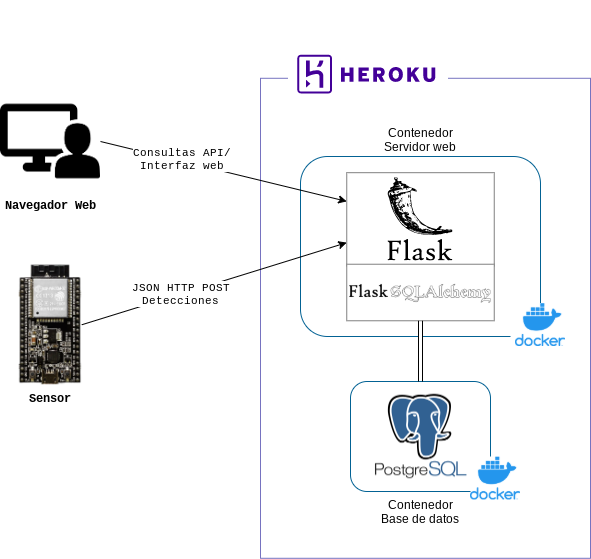
\includegraphics[scale=0.5]{implementacion/estructura_servidor_central}
\caption{Estructura servidor central }
\label{fig:estructura_servidor_central}
\end{figure}

\subsection{Base de datos}

El diseño de la base de datos para este proyecto ha resultado bastante sencillo siendo solo necesarias dos tablas, una para almacenar las detecciones y otra para los sensores a las que irán asociadas estas detecciones, en la Figura \ref{fig:table_diagram} se puede ver el contenido de estas tablas y su relación.

\begin{figure}[H]
\centering
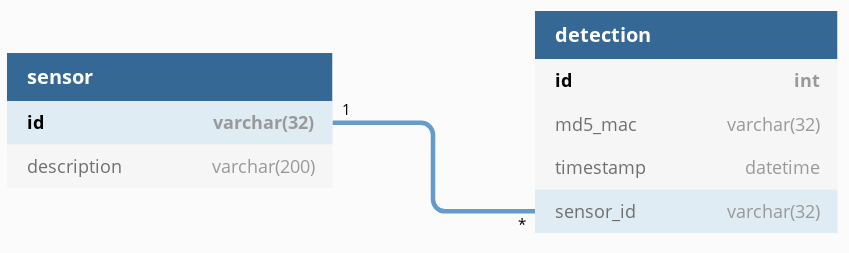
\includegraphics[scale=0.4]{implementacion/table_diagram}
\caption{Diagrama de Entidad-Relación del servidor central.}
\label{fig:table_diagram}
\end{figure}

Para facilitar la conexión con la base de datos y el tratamiento de los datos contenidos en ella se ha utilizado una librería ORM, de sus siglas en inglés \textit{Object Relational Mapper}, este tipo de librearías nos permiten mapear las estructuras de una base de datos relacional con objetos de un lenguaje de programación orientado a objetos, de forma que podemos acceder a tablas y filas de una base de datos como clases y objetos, además encapsula las sentencias SQL en forma de métodos, de esta forma no necesitaremos usar SQL para manipular los datos si no que interactuaremos directamente con objetos y métodos del mismo lenguaje que estamos usando, en este caso Python.\\

SQLAlchemy \cite{sqlalchemy} ha sido la herramienta ORM seleccionada para este fin, para integrarla con la aplicación se ha utilizado las extensión Flask-SQLAlchemy \cite{flask_sqlalchemy} que simplifica el uso de SQLAlchemy con Flask proporcionando valores predeterminados útiles y funciones adicionales que facilitan la realización de tareas comunes.\\

Utilizando esta extensión se han definido los modelos de datos utilizando clases dentro del código de la aplicación tal y como se muestra a continuación.\\

\begin{minipage}{\linewidth}
\begin{lstlisting}[language=Python, caption=Definición de modelos utilizando SQLAlchemy, label={lst:sqlalchemy_models}, captionpos=b, frame=single]
class Sensor(db.Model):
    id = db.Column(db.String(32), primary_key=True, index=True)
    description = db.Column(db.String(200))
    detections = db.relationship('Detection', backref='sensor', lazy=True)

    def __repr__(self):
        return 'Sensor {}, {}'.format(self.id, self.description)


class Detection(db.Model):
    id = db.Column(db.Integer, primary_key=True)
    md5_mac = db.Column(db.String(32), index=True)
    timestamp = db.Column(db.DateTime, nullable=False)
    sensor_id = db.Column(db.String(32), db.ForeignKey('sensor.id'), nullable=False)

    def __repr__(self):
        return 'Detection {}, MD5_MAC: {}, timestamps: {}, sensor: {}'.format(self.id, self.md5_mac, self.timestamp, self.sensor_id)
\end{lstlisting}
\end{minipage}

Para gestionar las migraciones de la base de datos se ha utilizado la extensión Flask-Migrate \cite{flask_migrate}, esta extensión genera scripts de migración con las instrucciones necesarias para reflejar los cambios de los modelos de datos de nuestro código en la estructura de la base de datos, además nos permite realizar un control de versiones de los cambios realizados en la estructura de la base de datos pudiendo volver a la versión anterior con un simple comando en caso de error.\\

\subsection{API REST}
Con el fin de permitir a los usuarios consultar las detecciones y sensores del sistema, además de permitir al sensor realizar inserciones de nuevas detecciones se ha desarrollado una API REST con Flask que expone tres \textit{endpoints}: \textit{sensors}, \textit{detections} y \textit{detections-collection}, para cada uno se han implementado los métodos más importantes en este tipo de APIs: consulta (GET), inserción (POST), modificación (PUT) y eliminación (DELETE); a excepción del \textit{endpoint detections-collection} que se detallará más adelante.\\

El acceso a la API se realiza a través del path \textit{/api/v1.0}, la última parte representa la versión de la API de cara a evitar problemas de retrocompatibilidad con los clientes debido a evolutivos que cambien, por ejemplo, los parámetros de entrada, en el caso de este proyecto solo está expuesta la versión mencionada.\\

A continuación se expone el listado de \textit{endpoints} expuestos junto a los métodos que implementan:\\

\noindent{\textbf{detections}}

\begin{itemize}
  \item \textit{GET /detections}:  Devuelve todas las detecciones realizadas.
  \item \textit{GET /detections/<detection\_id>}: Devuelve los datos asociados a una detección en concreto.
  \item \textit{POST /detections}: Crea una nueva detección.
  \item \textit{PUT /detections/<detection\_id>}: Modifica los datos asociados a la detección indicada.
  \item \textit{DELETE /detections/<detection\_id>}: Elimina la detección indicada.
\end{itemize}

\noindent{\textbf{detections-collection}}

\begin{itemize}
\item \textit{POST /detections-collection}: Creación masiva de detecciones.
\end{itemize}

\noindent{\textbf{sensors}}

\begin{itemize}
  \item \textit{GET /sensors}: Devuelve todos los sensores existentes.
  \item \textit{GET /sensors/<sensor\_id>}: Devuelve los datos asociados al sensor indicado.
  \item \textit{POST /sensors}: Crea un nuevo sensor.
  \item \textit{PUT /sensors/<sensor\_id>}: Modifica los datos asociados al sensor indicado.
  \item \textit{DELETE /sensors/<sensor\_id>}: Elimina el sensor indicado.
\end{itemize}

La información devuelta por estos \textit{endpoints} utiliza el formato de documentos JSON, igualmente el formato utilizado por los clientes para el envío de las peticiones de inserción y modificación (POST y PUT) es JSON. En el Código \ref{lst:json_detection} se puede ver un ejemplo del documento JSON para las detecciones y en el Código \ref{lst:json_sensor} para los sensores.\\

\begin{minipage}{\linewidth}
\begin{lstlisting}[caption=Ejemplo de JSON para detecciones, label={lst:json_detection}, captionpos=b, frame=single]
{
    "md5_mac": "874b165dccb840797ab7decdce8a3a40",
    "timestamp": "1598198020",
    "sensor_id": "f2946ea4a8712d3fb4e2253238da2632"
}
\end{lstlisting}
\end{minipage}

\begin{minipage}{\linewidth}
\begin{lstlisting}[caption=Ejemplo de JSON para sensores, label={lst:json_sensor}, captionpos=b, frame=single]
{
    "id": "363daf8619557863c7b4f9767389cb6c",
    "description": "ESP32 DevKitC"
}
\end{lstlisting}
\end{minipage}

Un caso especial es el del \textit{endpoint} para inserción masiva de detecciones \textit{/detections-collection}, este \textit{endpoint} está compuesto por un solo método \textit{POST} que nos permite realizar una creación masiva de detecciones con una sola llamada HTTP, este diseño atípico surge de las restricciones de tiempo de procesamiento del sensor para el envío de las detecciones ya que realizar una conexión HTTP por cada detección supondría una gran sobrecarga para el sensor, además para este método se ha diseño un formato de documento JSON simplificado prescindiendo de las claves de los valores de detección para reducir el uso de memoria en el sensor, en el Código \ref{lst:json_detecciones_masivas} se puede ver un ejemplo de documento JSON utilizado para realizar una inserción de múltiples detecciones.\\

\begin{minipage}{\linewidth}
\begin{lstlisting}[caption=Ejemplo de JSON para inserción masiva de detecciones, label={lst:json_detecciones_masivas},captionpos=b, frame=single]
{
  "node": "6e1142a5d86b1eca0ed13b408487fe05",
  "detections": {
    "70fbb859bf3606b8b0b54e30c2f1facd": 1563737210,
    "7598e7b767976cdd583135125da0836f": 1563737209,
    "9331c407b188128654e3c3c218bb10d8": 1563737215
  }
}
\end{lstlisting}
\end{minipage}

Para facilitar el tratamiento de los documentos JSON se ha utilizado la extensión Flask-Marshmallow \cite{flask_marshmallow}, esta extensión se integra con la extensión Flask-SQLAlchemy y nos permite crear esquemas (Código \ref{lst:marshmallow_schemas}) basados en nuestros modelos de datos  (Código \ref{lst:sqlalchemy_models}) facilitando la deserialización de los documentos JSON recibidos en objetos y viceversa, además nos aporta una capa de validación de los datos basándose en los tipos definidos en las clases de nuestro modelos.\\

\begin{minipage}{\linewidth}
\begin{lstlisting}[language=Python, caption=Esquemas de datos de Flask-Marshmallow, label={lst:marshmallow_schemas},captionpos=b, frame=single]
class DetectionSchema(ma.ModelSchema):
    class Meta:
        model = Detection
        # Fields to expose
        fields = ("id", "md5_mac", "timestamp", "sensor_id")

    @pre_load
    def convert_timestamp(self, in_data, **kwargs):
        in_data['timestamp'] = str(datetime.fromtimestamp(float(in_data['timestamp'])))
        return in_data


class SensorSchema(ma.ModelSchema):
    class Meta:
        model = Sensor
        # Fields to expose
        fields = ("id", "description")

detection_schema = DetectionSchema(dump_only=["id"])
detections_schema = DetectionSchema(many=True)
sensor_schema = SensorSchema(dump_only=["detections"])
sensors_schema = SensorSchema(many=True)
\end{lstlisting}
\end{minipage}

Esta extensión nos permite reducir considerablemente el código necesario para tratar las peticiones a la API, en el Código \ref{lst:marshmallow_example} se muestra como ejemplo el tratamiento de la llamada a la API para crear un nuevo sensor, se puede observar como con una sola línea se realiza la validación y deserialización del documento JSON de entrada a un objeto de nuestra base de datos.\\

\begin{minipage}{\linewidth}
\begin{lstlisting}[language=Python, caption=Ejemplo de funcionamiento de Flask-Marshmallow, label={lst:marshmallow_example},captionpos=b, frame=single]
@api.route('/sensors/', methods=['POST'])
def new_sensor():
    sensor = sensor_schema.load(request.json, session=db.session).data}
    db.session.add(sensor)
    db.session.commit()

    return sensor_schema.jsonify(sensor), 201, \
           {'Location': url_for('api.get_sensor', sensor_id=sensor.id)}
\end{lstlisting}
\end{minipage}

\subsection{Frontal Web}

Para el diseño del frontal se  ha utilizado el \textit{framework} Bootstrap \cite{bootstrap_frontend_framework}, este \textit{framework} nos permite un desarrollo rápido y sencillo de interfaces web combinando CSS y Javascript, para ello nos facilita plantillas de diseño y elementos prediseñados como botones, formularios o menús de navegación. Además estos elementos están pensados para el diseño web adaptativo (\textit{responsive}) por lo que se ajustan de forma nativa a distintas resoluciones facilitando su visualizado en diferentes tipos de dispositivos. Para facilitar su integración con el motor de plantillas Jinja 2 se ha utilizado la extensión \textit{Flask-Bootstrap} \cite{flask_bootstrap} que proporciona macros para evitar repetir código innecesariamente a la vez que nos permite personalizarlo.\\

También se ha utilizado \textit{Flask-Paginate}, esta extensión nos facilita herramientas para realizar la paginación de las detecciones mostradas en la interfaz web, necesario dado el gran volumen de detecciones a mostrar, para ello esta extensión nos proporciona los mecanismos para controlar la cantidad de elementos que se consultarán a la base de datos en cada vista, además de funciones para la generación de los elementos HTML necesarios para facilitar la navegación al usuario. \\

El resultado del uso de estas herramientas es una interfaz web limpia y sencilla que nos permite visualizar los sensores y las detecciones realizadas cómodamente tal y como se muestra en las Figuras \ref{fig:interfaz_web_detecciones} y \ref{fig:interfaz_web_sensores}.\\

\begin{figure}[H]
\centering
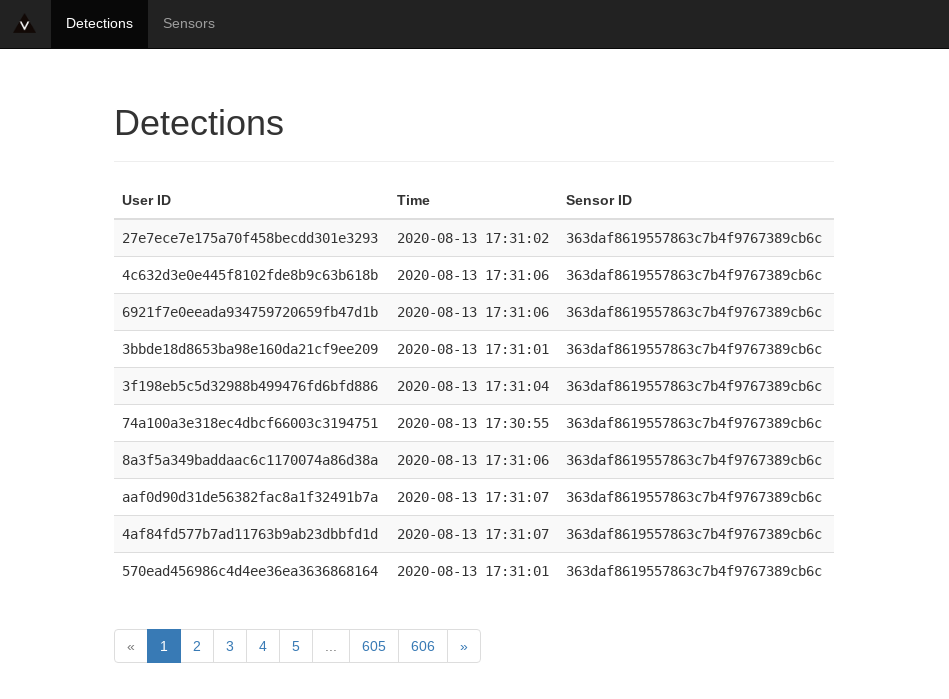
\includegraphics[scale=0.32]{implementacion/interfaz_web_detecciones}
\caption{Interfaz web de visualización de detecciones}
\label{fig:interfaz_web_detecciones}
\end{figure}

\begin{figure}[H]
\centering
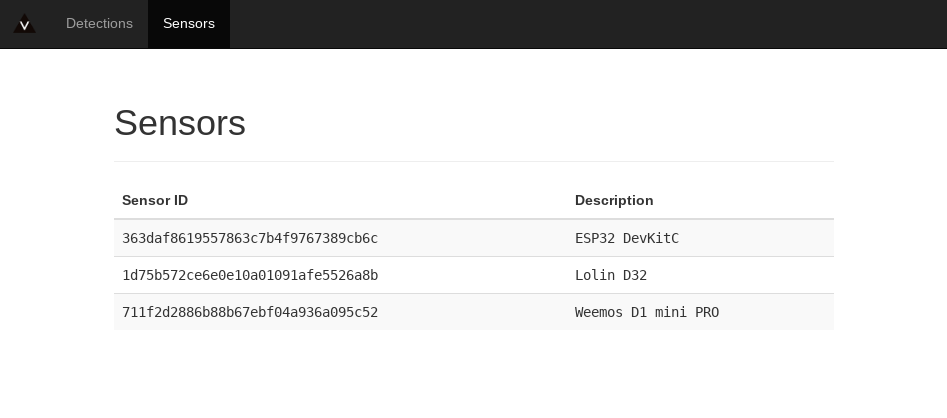
\includegraphics[scale=0.32]{implementacion/interfaz_web_sensores}
\caption{Interfaz web de visualización de sensores}
\label{fig:interfaz_web_sensores}
\end{figure}

\subsection{Herramientas de despliegue}

\subsubsection{Docker}

La primera pieza de este despliegue es la definición del contenedor que ejecutará la aplicación web, esta definición se realiza mediante el fichero \textit{Dockerfile} que contiene las instrucciones necesarias para crear la imagen que ejecutará el contenedor, como se puede observar en la primera línea del \textit{Dockerfile} para esta imagen se ha decidido partir de una imagen ya existente, \textit{python:alpine}, que nos proporciona una instalación base de Python sobre el sistema operativo ligero \textit{Alpine}, a partir de esta se instalarán las dependencias necesarias para ejecutar la aplicación y se copiará el código de la propia aplicación, entre otras acciones.\\

\begin{minipage}{\linewidth}
\begin{lstlisting}[caption=Dockerfile del servidor web, captionpos=b, frame=single]
FROM python:alpine

EXPOSE 5000

ENV VIRTUAL_ENV=/opt/venv

RUN adduser -D vedetra

WORKDIR /home/vedetra

COPY requirements.txt requirements.txt

RUN apk --update add --no-cache --virtual .build-deps \
    gcc \
    musl-dev \
    postgresql-dev \
 && apk --update add --no-cache postgresql-client \
 && python -m venv "$VIRTUAL_ENV" \
 && ${VIRTUAL_ENV}/bin/pip install --no-cache-dir -r requirements.txt \
 && apk del --no-cache .build-deps

USER vedetra

COPY app app
COPY tests tests
COPY migrations migrations
COPY vedetra-server.py config.py  entrypoint.sh ./

ENTRYPOINT ["./entrypoint.sh"]
\end{lstlisting}
\end{minipage}

Para el contenedor de PostgreSQL al no ser necesaria ninguna modificación se ha decidido utilizar directamente la imagen oficial de PostgreSQL (\textit{postgres:11-alpine}) sin necesidad de definir un fichero \textit{Dockerfile}, simplemente será necesario definir como variables de entorno el usuario y contraseña que la aplicación web utilizará para conectarse, el script de inicio que incluye esta imagen se encargará de crear dicho usuario.\\

Una vez definidas las piezas básicas de este despliegue es necesario componer un servicio con ellas, para ello se ha utilizado Docker Compose, es una herramienta que permite definir y ejecutar aplicaciones basadas en múltiples contenedores Docker, para definir este servicio se utiliza un fichero YAML denominado \textit{docker-compose.yml}, en este fichero se define el origen o generación de las imágenes, la dependencia entres los contenedores, como se comunican entre ellos y con el exterior y las variables de entorno que se insertarán en los contenedores. \\

\begin{minipage}{\linewidth}
\begin{lstlisting}[caption=Fichero docker-compose.yml base, captionpos=b, frame=single]
version: '3'
services:
  vedetra:
    build: .
    ports:
      - "5000:5000"
    env_file:
      - web.env.sample
    depends_on:
      - "db"
  db:
    image: "postgres:11-alpine"
    restart: always
    env_file: db.env.sample
    expose:
      - 5432
\end{lstlisting}
\end{minipage}

Esta definición nos permite utilizar Docker Compose para desplegar todo el entorno con el simple comando \textit{docker-compose up}.\\

Docker Compose también nos facilitá la posibilidad de personalizar una aplicación para  diferentes entornos sin tener que reescribir la definición para cada entorno, para ello nos permite utilizar varios ficheros \textit{compose} que se combinarán, en el fichero base \textit{docker-compose.yml} se establece la definición común a todos los entornos y en un segundo fichero se definen las directivas específicas del entorno que ampliarán o sobreescribirán las definidas en el fichero base, por ejemplo, en el entorno de desarrollo se define un fichero de variables de entorno diferente y se añade un volumen al contenedor que estará conectado a la carpeta local del proyecto de forma que podamos realizar modificaciones en el código sin necesidad de recrear la imagen.\\

\begin{minipage}{\linewidth}
\begin{lstlisting}[caption=Fichero docker-compose.yml para el entorno de desarrollo, captionpos=b, frame=single]
version: '3'
services:
  vedetra:
    env_file:
      - "web-dev.env"
    volumes:
      - .:/home/vedetra
  db:
    env_file: "db-dev.env"
\end{lstlisting}
\end{minipage}

\subsubsection{Heroku}

Para tener una mayor consistencia entre los entornos de desarrollo y producción se ha utilizado la funcionalidad de despliegue con contenedores de Heroku, esta funcionalidad nos permite construir la imagen del contenedor automáticamente al subir el código al repositorio de Heroku, tan solo es necesario definir la ubicación del Dockerfile que se usará para construir el contenedor.\\

\begin{minipage}{\linewidth}
\begin{lstlisting}[caption=Definición de aplicación de Heroku, captionpos=b, frame=single]
build:
 docker:
   web: Dockerfile
\end{lstlisting}
\end{minipage}

Heroku no permite el uso de Docker Compose por lo que no podemos hacer un despliegue multicontenedor, por este motivo para el componente de la base de datos se ha utilizado el \textit{addon} Heroku PostgreSQL que nos permite desplegar una base de datos PostgreSQL con un simple comando.\\

\end{document}
